\chapter{The Proposed System}
\label{sec:proposedSystem}
\section{Aims of the System}
\label{sec:AimsOfTheSystem}
%The previous chapter showed the current trends in sketch recognition. 
This thesis introduces a new approach for the sketch recognition problem. Particle Swarm Optimization (PSO) is used to correctly segment strokes into curves and lines. The current implemented systems either segment strokes based on simple curvature\cite{meanshift10,earlySketchbased4} or speed information\cite{earlySketchbased4}.


The contribution in the system is mainly in attempting to generate the optimal segmentation using PSO which exhibited superiority with respect to similar algorithms in various other applications \cite{PolygonApproximationPSO}. The system attempts to find the optimal decomposition of the input stroke using PSO with the help of curvature and speed information. The use of PSO algorithm helps in eliminating the effects of input noise, problems of over and under segmentation that were in pervious systems. The proposed symbol recognizer uses the generated segmentation to compute the feature vector which is used to identify more complex symbols. This enables the system to be scalable for more  complex shapes.


 %the performance of most algorithms is based on user style. 

% Stroke segmentation is one of the most complex problems in the sketch recognition system. It is dividing the   
%In stroke segmentation problem is Particle swarm optimization is used as the 

\section{System Overview}
\label{sec:AnOverviewOfTheSystem}
   This research solves sketch segmentation problem using particle swarm algorithm (PSO).  Due to sloppiness of users and hardware glitches the captured points must be processed to remove noise and redundancy before the system proceeds to compute the speed and curvature information. After that a set of possible corner or critical points is computed to guide the segmentation procedure.  A set of features is extracted from the segmented strokes to be used by the classifier.  %The stroke is the path of points from the instant the pen is down till it is up.
The block diagram in Figure \ref{fig:Blockdiagram} shows the main system blocks. The next section describes each block in details.
 %Due to sloppiness of users and hardware glitches the system processes the data before further
\begin{figure}[]
	\centering
	
\begin{center}
	\includegraphics[scale=0.75]{images/AllBlockDiagram.eps}
	\caption[The System Block Diagram]{Block diagram of the system}
	\label{fig:Blockdiagram}
\end{center}
\end{figure}
 

%\subsection{System Components}
%\label{sec:SystemComponents}

The \textbf{preprocessing} step is responsible for capturing the input data and removing the noise from it. As shown in Figure \ref{fig:Blockdiagram} preprocessing consists of computing the time differences, direction, speed and curvature of every point in the stroke. After computing this information the local minimum and local maximum of each curve is extracted. This process estimates a set of a set of Possible Dominant Points $P_{pd}$ that guide the segmentation process. Later, other geometrical and statistical computations are evaluated from the stroke. %The system then proceeds to estimate to help in the segmentation process.   \\
 
  
The next step is \textbf{Segmentation}, the goal of the segmentation stage is to divide strokes into segments of either curves or lines. The segmentation problem is summarized as finding the best decomposition with least number of segments each represents a geometric primitive. This is an optimization problem, which evolutionary programming can solve efficiently. A genetic algorithm was used by \cite{CruveDivisionSwarm} to optimally divide digital curves into lines and curves. Chen et al.\cite{CruveDivisionSwarm} uses digital curves scanned from paper as input to the system and did not take advantage of the curvature or local geometric properties of the digital curve.

 As shown in Figure \ref{fig:Blockdiagram} first an attempt is made to fit the stroke points into a curve or an ellipse using a minimum square error fitting algorithm \cite{chernov-2003}. If the stroke proved to be an elliptical arc then the segmentation process ends and the system proceeds to the next step. Otherwise, the stroke is passed to two particle swarm algorithms that divide the stroke to either a polygon or a set of lines and curves. The algorithms takes the stroke points along with the possible dominant points $P_{pd}$ computed during preprocessing then produce a set of dominant points which are connected by either lines or curves. The two algorithms will generate two segmentations, the system will choose the segmentation that has the minimum segmentation error.%
% First an attempts the segmentation process is divided into two steps ellipse fitting and curve segmentation. In the first step, the ellipse fitting process tries to fit the stroke into an ellipse. If the system fails it passes the stroke to the second step; curve segmentation which consists of two PSO segmentation algorithms. The two algorithms will generate two segmentations, the system will choose the segmentation that has the minimum segmentation error.%  generate the segmentations,  the minimum error will be the chosen segmentation. % is the ellipse fitting

 %the stroke first If the ellipse detection fails the stroke is passed to the segmentation algorithms which will pass it to the two PSO algorithms described below the segmentation with the minimum error will be the chosen segmentation.  The segmentation is then added to the set of un-recognized segments in the system. \\% this part is repeated for each stroke. 
 %the clustering algorithm starts to group segments together after the segmentation step. The system let the user draws the symbol by using any number of strokes, a set of unrecognized segments is passed to the clustering algorithm to generate a symbol and compute a feature vector for it.
 
 In \textbf{Feature Extraction} step, a feature vector consists of a set of statistical, geometrical and spatial features are extracted from the segmented strokes. The feature vector is used as input for the next step.   %the system computes composite set of features some are statistical other are spatial features based on the type primitives.% The system extract segment based and statistical based features from the set of segments that the clustering algorithms produce. 
  
   The final step is \textbf{Classification} using a SVM classifier. The classifier attempts to classify the symbol into one the previously trained classes.% c  that will use the features computed to classify the segments into one of the previously trained classes. % Or to determine the symbol of the given segments from the set of preciously trained symbols. 
 
 %with a symbol from the training set.% The system compute composite set of features some are statistical other are spatial features based on the type primitives. Finally, the strokes are classified into the corresponding classes.% the classifier identifies the strokes into a symbol from the set of known symbols.\\

%\chapter{System Details}
%\label{sec:SystemDetails}


\section{Preprocessing}
\label{sec:Preprocessing}
%Some data is extracted from the points in the stroke.
The preprocessing step captures the points from the pointing devices then compute the information needed to determine a set of  \textit{Possible Dominant Points $P_{pd}$} which guides the segmentation step. It is noted as a person draws a shape the pen slows down near corners and picks up speed when drawing straight lines. Therefore, the speed information is widely used to identify the shape corners and edges \cite{earlyprocess}. The curvature information is used to determine the points with high angular changes along the path of points \cite{meanshift10}. Those observations help detecting the dominant points as the points with lower speeds and high curvatures. 

Also the time difference between samples was used in \cite{polygonfeedback31} as it provides more distinct maxima than the speed information. Agar et al. \cite{polygonfeedback31} mentions that the pointing device (for example the mouse) sampling rate is the reason for this phenomena. The points are sampled at regular time intervals while the pointing device is moving. There are no points while the pointing device is stationary. This leads to a nearly constant time difference between samples while the pen is moving and large difference while the pen is stationary. Contrary to speed information, where the users draw with variant speeds the speed information has a lot of noise in the data. Figure \ref{fig:speed2Distance} shows the time difference and the speed graphs for the stroke drawn in Figure \ref{fig:orignalStroke}.  Similarly, direction information is used as it provides better distinctive maxima for the corners than the curvature information \cite{meanshift10}. Figure \ref{fig:curvatures} shows the direction and curvature graphs for the stroke drawn in Figure \ref{fig:orignalStroke}

 %The system compute speed, curvature, time difference and direction data then generate a set of possible corners that will be used in the segmentation as an initial solution. 
\subsection{Preliminary Calculation}
\label{sec:CurvatureCalculation}
  
 
 In this research, time difference, direction, speed and curvature of each point along the stroke was computed. The experiments in section \ref{sec:PSO} proved that computing all information's provide better segmentations results than only using one of the graphs. The time difference is calculated as $\Delta t = t_{i+1} - t_i$ where $t_i$ is the time of the point $i$ and $t_{i+1}$ is the time of the point $i+1$. The speed is calculated using equation $v=\Delta s/\Delta t$ where $t$ is the time difference between two points and $s$ is the length between them. 
 
\begin{figure}
	\centering
		\includegraphics{images/curvatureCal.jpg.eps}
	\caption{Direction Calculation}
	\label{fig:curvatureCal.jpg}
\end{figure}

  The direction is calculated as the angle between vectors $Q_i$ and the $x-axis$ (vector $O_i$) as in equation \ref{eq:direction} (Figure \ref{fig:curvatureCal.jpg} explains direction calculations).We used a n estimation of curvature that define curvature as the change in direction with respect to length i.e. $c= \Delta d/\Delta s$.
  
 \begin{equation}
\label{eq:direction}
	\vartheta  = \cos ^{ - 1} \left( {\frac{{\overrightarrow {Q_i}  \cdot \overrightarrow {Px_i } }}{{\left\| {\overrightarrow {Q_i} } \right\| \times \left\| {\overrightarrow {Px_i} } \right\|}}} \right)
\end{equation}
where $Q_i=\overrightarrow {P_{i - 1} P_i }$ is the vector from the point  $P_{i - 1}$ to point $P_i$ and $Px_i$ represent the $x-axis$ at this point (Figure \ref{fig:curvatureCal.jpg}).  $\|{\overrightarrow {Q_i }}\|$ is the normal of the  vector $\overrightarrow{Q_i}$
 
 
 
 %system compute speed, distance data for all points in the stroke. Curvature is computed using estimation used in [] where direction computed is angle between two lines. Curvature is 
 %$\Delta d/  \Delta S $ where d is the difference direction of point and s is difference in distance between points. 
 All these calculations are performed in real time while the user draws the strokes. The complexity of computation is $O(n)$ where $n$ is number of points. Figures \ref{fig:speed2Distance} \&  \ref{fig:curvatures} show the computed information's for the stroke drawn in Figure \ref{fig:AnotherorignalStroke}.% After computing the graphs the system  compute the average, minimum and maximum values of all curves.  \\% the lower speed points correspond to vertex and dominant point's location. The higher the direction and curvature data correspond to location with higher change in curvature witch promote the location for vertices'. \\
%Description of input data. 
%how to calculate speed, curvature, area, bounding box.
%how to remove noise. 
%Finally how to compute primarily dominant points. 

\begin{figure}[]
	\centering
		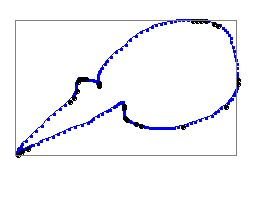
\includegraphics[scale=0.8]{images/stroke3.jpg.eps}
	\caption{Example of Input Stroke} Example of an input stroke to the system. 
	\label{fig:orignalStroke}
\end{figure}


\begin{figure}
	\centering
			\subfigure[ Speed Graph]{	\includegraphics[scale=0.5]{images/vel3orginal.png.eps}}
			\hfill
			\subfigure[ Time Difference Graph] {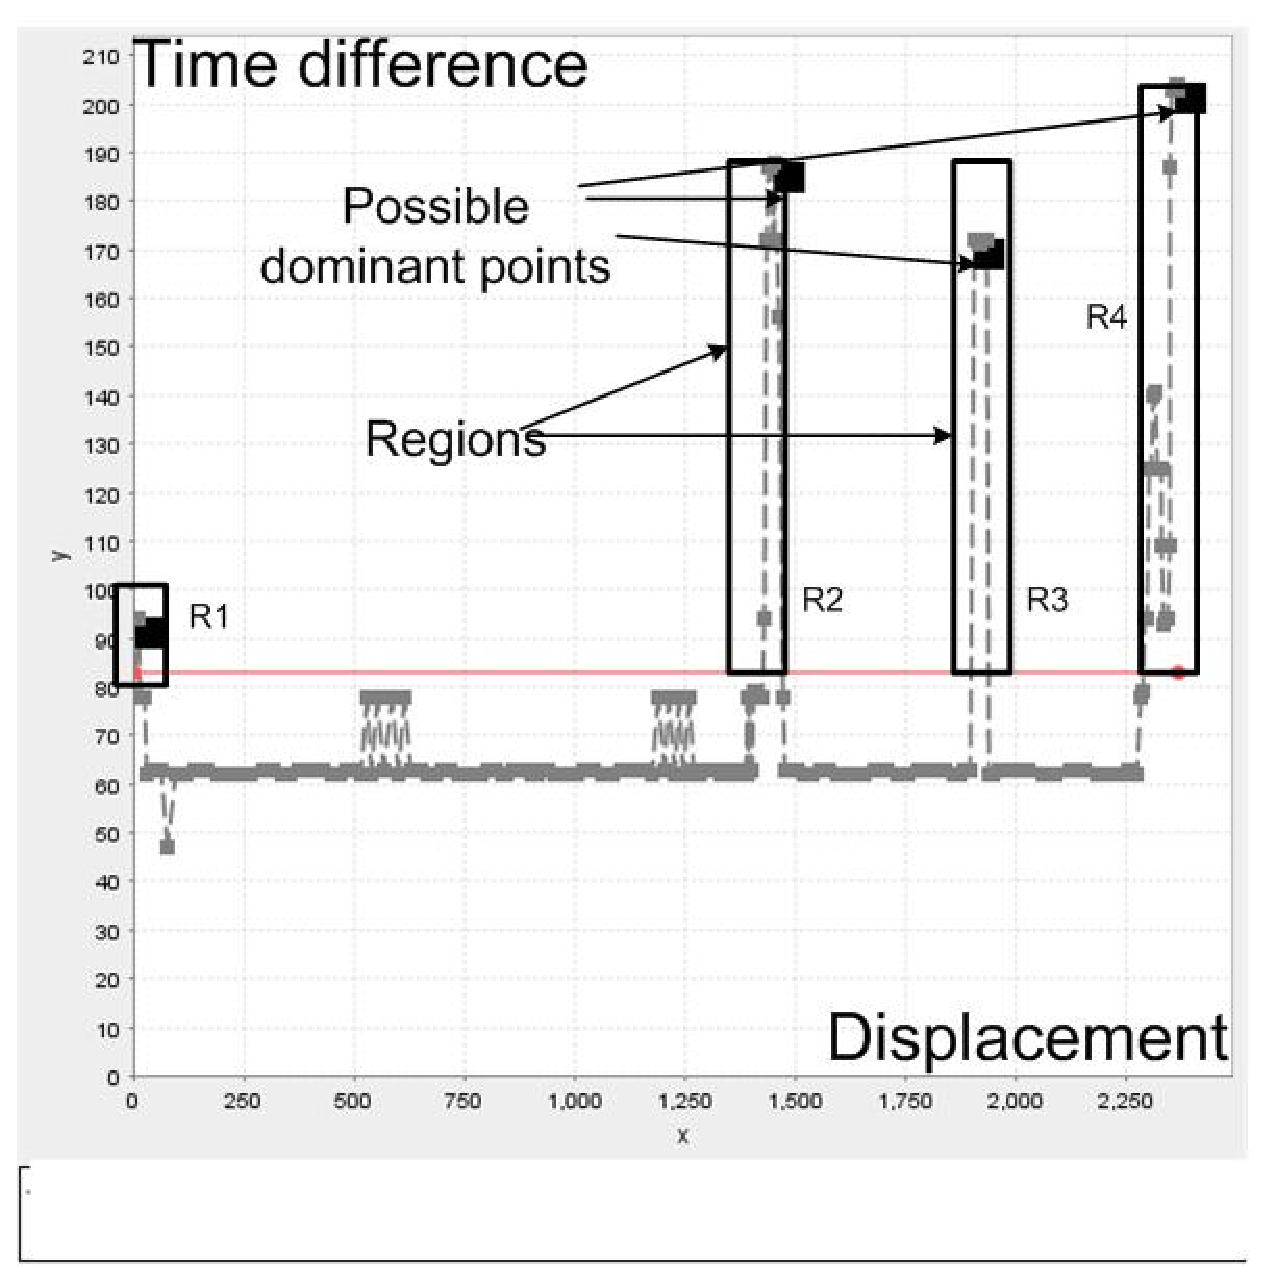
\includegraphics[scale=0.5]{images/td3.jpg.eps}}
	\caption{Speed and Time Difference Graphs}
	\label{fig:speed2Distance}
\end{figure}

\begin{figure}[]
	\centering
		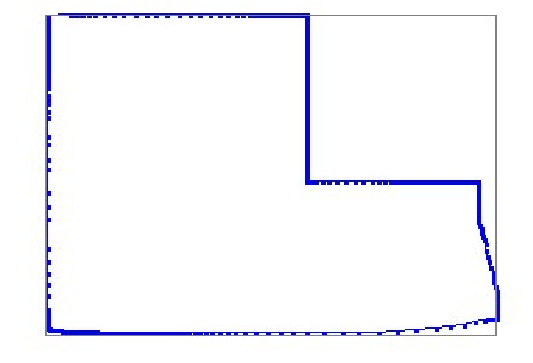
\includegraphics[scale=0.8]{images/orignalStroke.eps}
	\caption{Another Example of Input Stroke} Example of an input stroke to the system. 
	\label{fig:AnotherorignalStroke}
\end{figure}

\begin{figure}[]
%\begin{minipage}[b]{0.8\linewidth}
	\centering

	%	\subfigure[ The Speed of data] {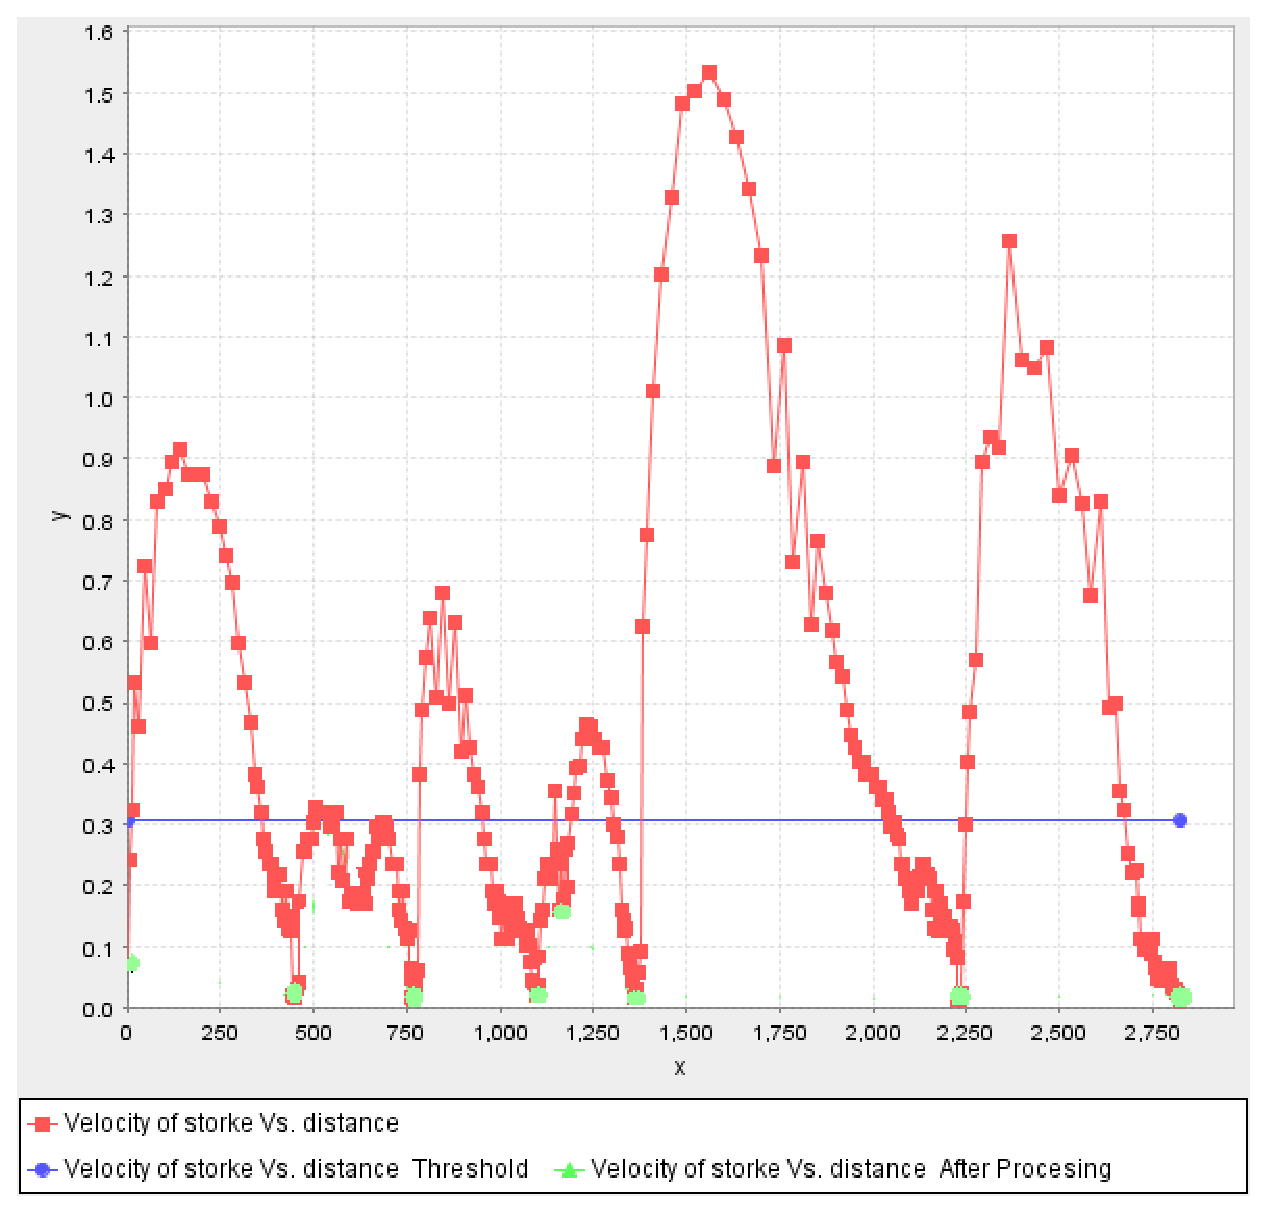
\includegraphics[scale=0.35]{images/speed2.eps}}
		
		\subfigure[ Direction Graph ] {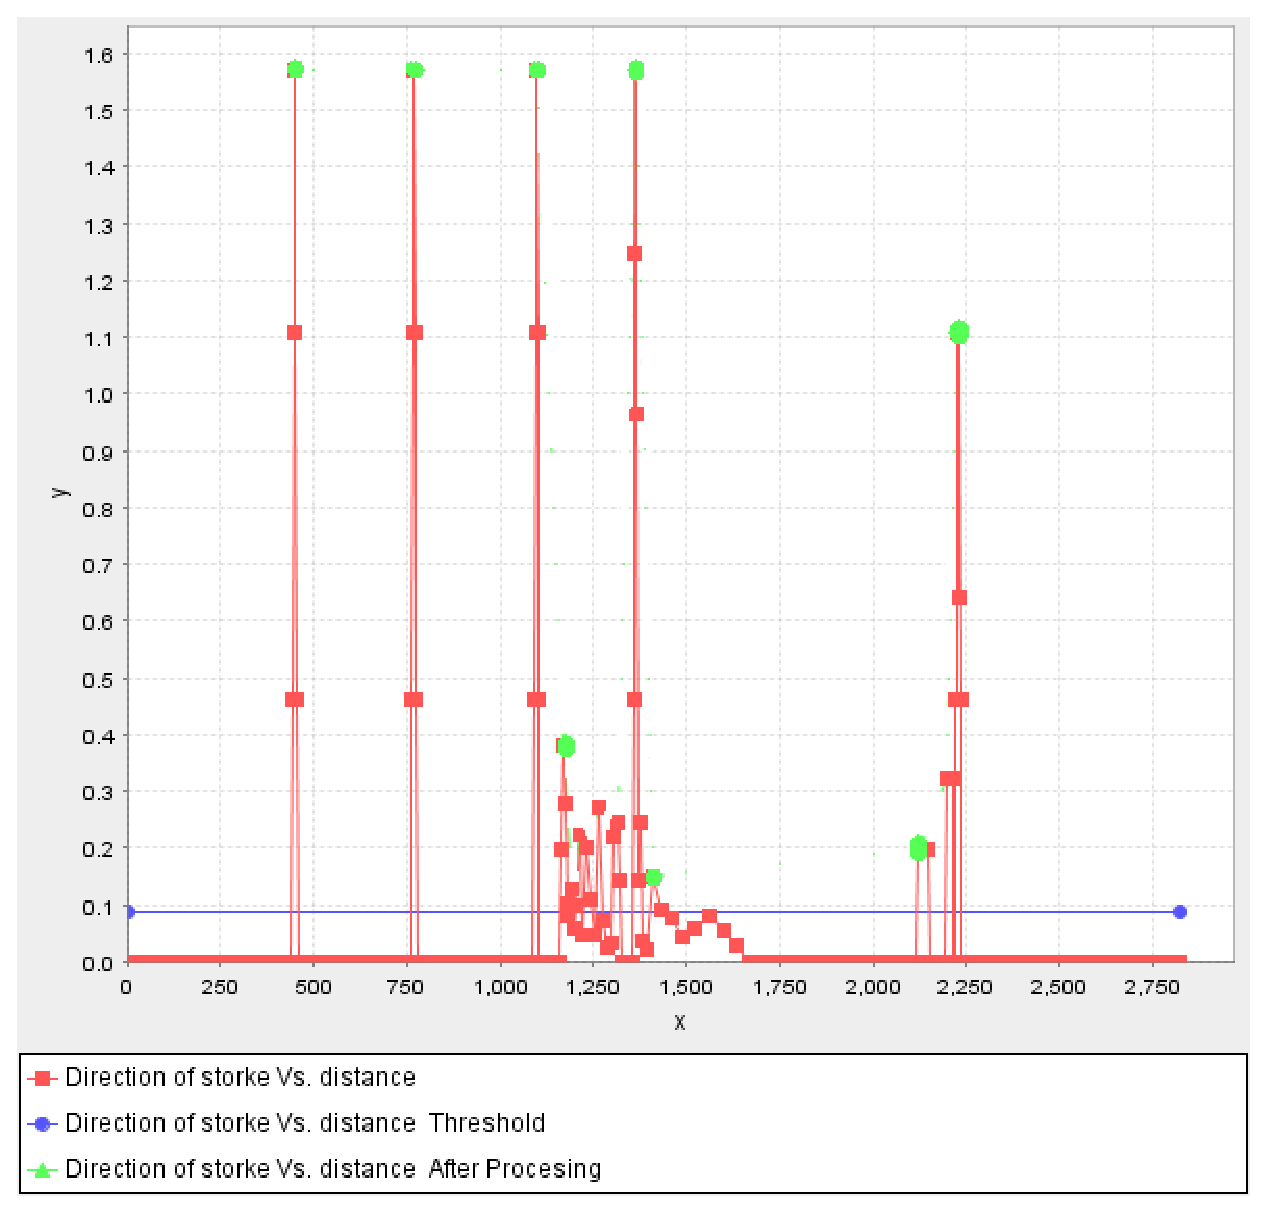
\includegraphics[scale=0.35]{images/direction2.eps}}
					%\end{minipage}
					%\begin{minipage}[b]{0.8\linewidth}
			\subfigure[Curvature Graph] {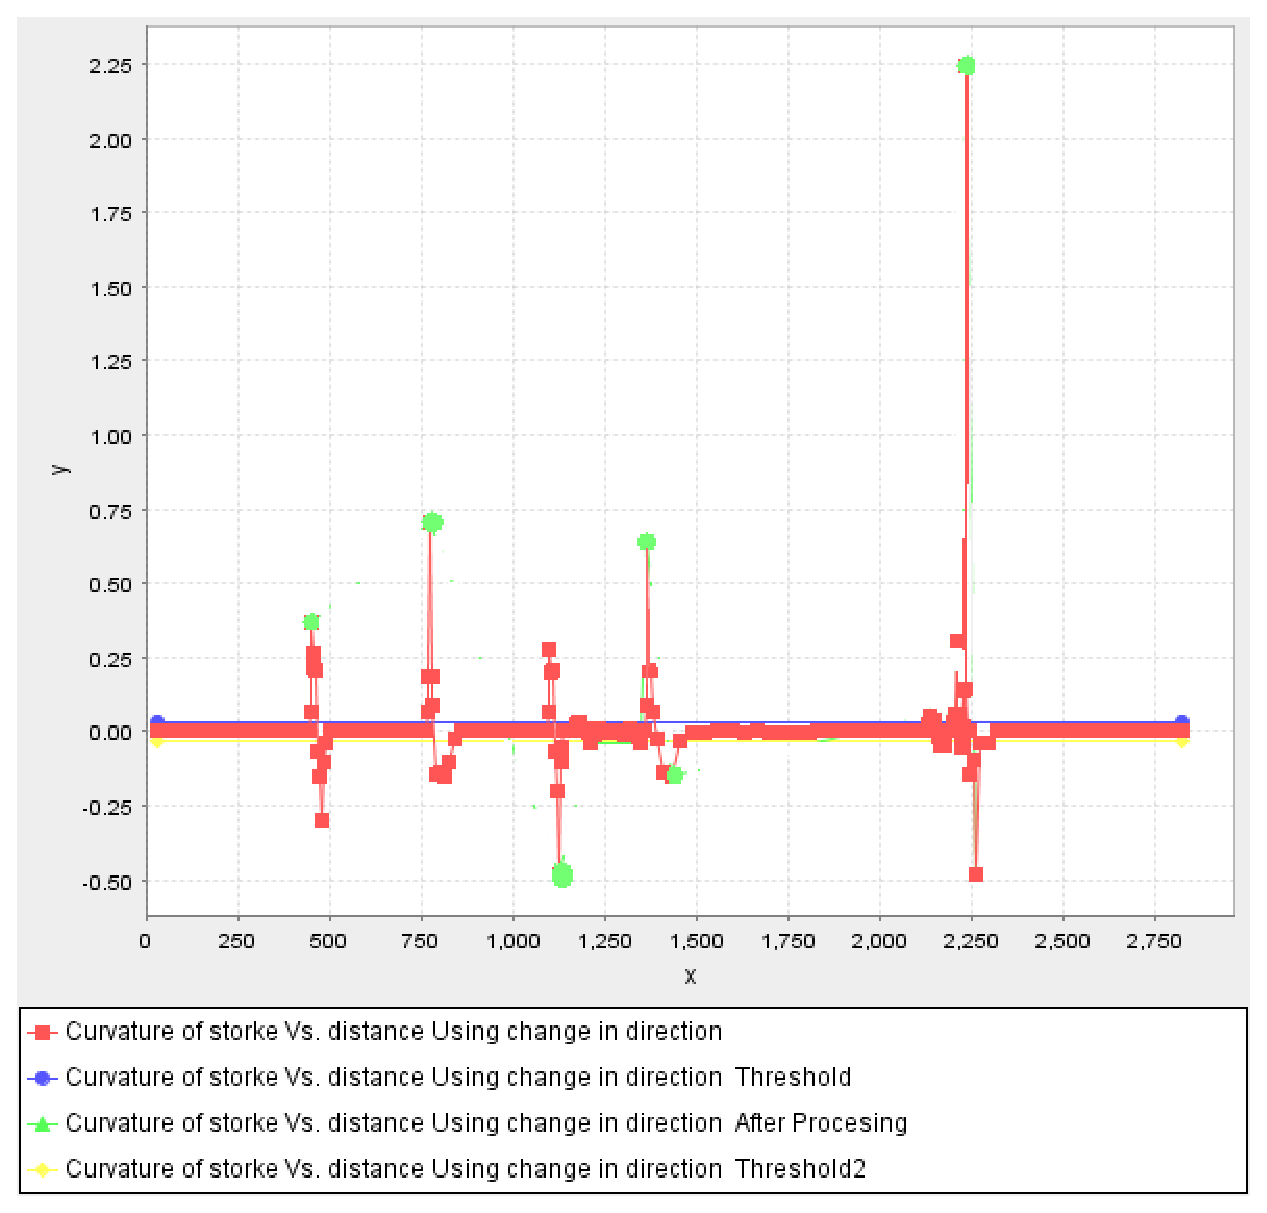
\includegraphics[scale=0.35]{images/curvature2.eps}}
		
			%\end{minipage}
	
	\caption{Curvature and Direction Graphs}%{The data of the stroke}
	
	\label{fig:curvatures}
\end{figure}


\subsection{Critical Point Detection}
\label{sec:CriticalPointDetection}
After computing speed, time difference and curvature information the system proceeds to detect the points with low velocity and high curvatures. Using simple differentiation to detect local extreme points resulted in false points due to the non smooth curves. Hence, the system adopted a process presented by \cite{earlyprocess}, where the mean of the curve is calculated. Then a threshold \textit{th} is used to separate the curve into regions; each region $Region_i$ is defined as a range of points, where the curve values are either above or below the threshold \textit{th}. Those regions are further processed to find the maximum point $Max(Region_i)$ of each region $Region_i$. The stroke points $p_i(x,y)$ that correspond to those maximum values are labeled as \textit{possible dominant points} $P_{pd}$. Figure \ref{fig:MaxRegioi} and \ref{fig:speed2Distance} shows an example of $Region_i$ of the speed curve and the dominant points $P_{pd}$ which correspond to the minimum of point in this region $Min(Region_i)$.  % (as shown are redundant)
\begin{figure}
	\centering
		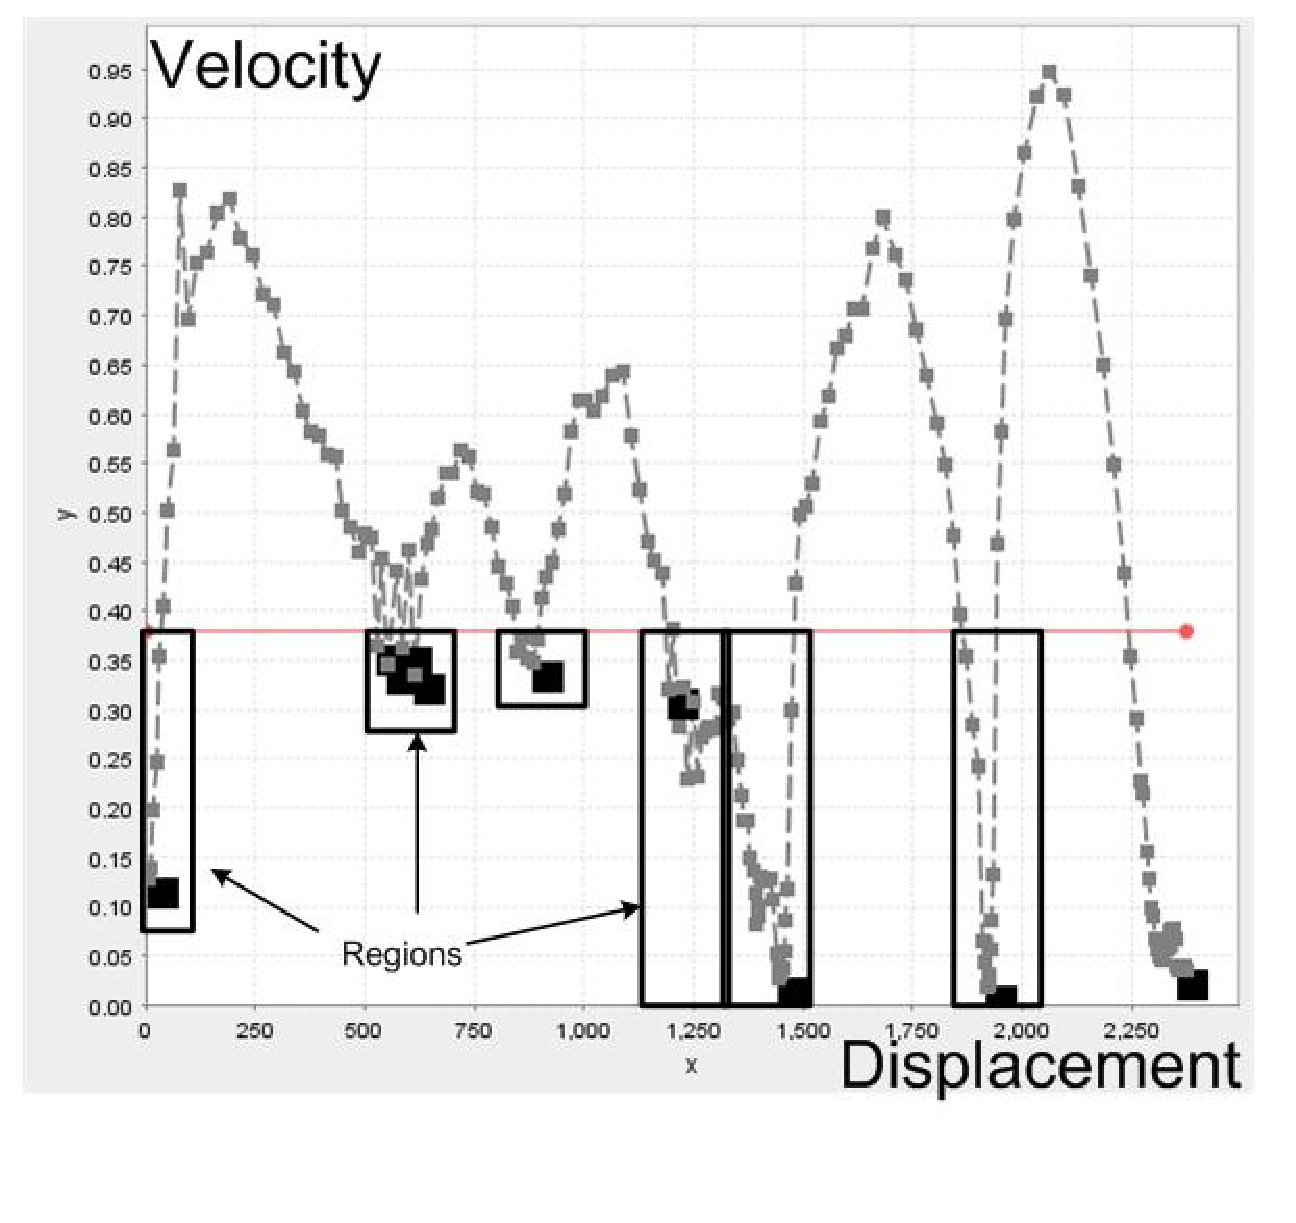
\includegraphics[scale=0.5]{images/vel3.jpg.eps}
	\caption{Possible Dominant Points Calculations}
	\label{fig:MaxRegioi}
\end{figure}

   %After the threshold is applied the curve is divided into regions. Each region is defined by a part in the data curve between tow intersection point of the threshold line and the curve.  % to find the extreme points. Hence, the mean of the direction curve is calculated and used as threshold.   \\
   %If we tried to differentiate the curve the result will be false threshold values we divide the data into regions of data higher or lower that the threshold. This will let us only look for high data only. The maximum of each region is then computed and reported as a possible vertex point. 
  
The system repeats this process to curvature, direction, time difference and speed curves. For each curve the points labeled as possible dominant points $P_{pd}$ are saved into a single array. The points that are repeatedly labeled are given a higher score than the other points. This score is then used to sort the  $P_{pd}$ points array. The array that contains possible points $P_{pd}$ is used as input for the next segmentation step. Figure \ref{fig:LabelsPPD} shows the particles labeled as Possible dominant points $P_{pd}$ by the preprocessing, it is noticed the redundancy of some $P_{pd}$ points. 


\begin{figure}
	\centering
		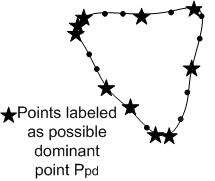
\includegraphics{images/ppd.eps}
	\caption{Possible dominant points}% a) Possible dominant point b) Particle encoding  
	\label{fig:LabelsPPD}
\end{figure}

\section{Segmentation}
\label{sec:Segmentation}
The segmentation tries to divide the stroke into a set of primitives. As shown in Figure \ref{fig:Blockdiagram} first an attempt is made to fit the stroke points into a curve or an ellipse using a minimum square error fitting algorithm \cite{chernov-2003}. If the stroke proved to be an ellipse arc then the segmentation process ends and the system proceeds to the next step. Otherwise, the stroke is passed to two particle swarm algorithms that divide the stroke to either lines or lines and curves. The algorithms take the stroke points along with the possible dominant points $P_{pd}$ computed during preprocessing then produce a set of dominant points which are connected by either lines or curves. The next section describes the ellipse detection algorithm and the two particle swarm algorithms used to divide the stroke.
%If the stroke proved to be an ellipse then the segmentation process ends and the system proceeds to the next step. Otherwise, the stroke is passed into two particle swarm algorithms that will divide the stroke to either lines or lines and curves (see the block diagram in fig. \ref{fig:Blockdiagram} ). 
%The algorithms takes the stroke points along with the possible dominant points computed then produce a set of dominant points which are connected with either lines or curves (see fig. \ref{fig:Blockdiagram}).  The next sections will describe the ellipse detection algorithm and both the two particle swarm algorithms used to divide the stroke.
%After computing the primary data the system now tries \\
%Paragraphs describe the segmentation algorithm.  


\subsection{Ellipse Fitting }
\label{sec:EllipseDetection}

%The process starts by computing the center of the stroke bounding box. The bounding box center point is used as the first estimation of the ellipse center. The axes of the ellipse are estimated as $width/2$ and $height/2$ of the stroke bounding box. The least square fitting algorithm is used to minimize the fitting error of the ellipse equation \cite{chernov-2003}.  
This process tries to fit the stroke points into an ellipse arc; it starts with computing the center of the stroke bounding box. The bounding box center point is used as the first estimation of the center of the ellipse. The axes of the ellipse are estimated as the $width/2$ and $height/2$ of the stroke bounding box where $width$ is width and $height$ is height of the bonding box. The least square fitting algorithm \cite{chernov-2003} is used to minimize the fitting error of the ellipse Equation (\ref{eq:circleFit})  

\begin{equation}
E = \sum\limits_{i = 0}^N {\frac{{(x_i - x_0 )}}{{a^2 }}^2  + \frac{{(y_i - y_0 )}}{{b^2 }}^2  - 1} 
\label{eq:circleFit}
\end{equation}

 where $N$ is number of points in the stroke, $a,b$ are the length of ellipse axes, $x_0$ \& $y_0$ are the coordinates of the center point, $x_i$ \& $y_i$ are the coordinates of point $i$ in the stroke. A list of new values for $x_0$ , $y_0$ ,$a$ and $b$ are generated randomly from the older values with small increments after each loop.  After few iteration, the final fit error of the estimated ellipse is reported. Another measure is used to compute the efficiency of the final estimated ellipse. Equation \ref{eq:circleError} ensures that the drawn percentage of ellipse is considered. This eliminates fitting a  line into very large ellipse but leaves small ellipses to be fitted as a partial or full ellipse. 


  \begin{equation}
eff = \left\{ {\begin{array}{*{20}c}
   {\frac{{P_{percent} }}{E}} & {ifP_{percent}  < 0.5}  \\
   {\frac{{P_{percent} }}{{E \times 2}}} & {ifP_{percent}  \ge 0.5}  \\
\end{array}} \right.
%eff= \begin{cases} 
% \frac{P_{percent}}{E},&\mbox{if} P_{percent}\mbox{< 0.5} \\
% \frac{P_{percent}}{2\times E},&\mbox{if} P_{percent}\mbox{\geq0.5} 
%\end{cases}
\label{eq:circleError}
\end{equation}
 \begin{equation}
P_{percent}  = L_{stroke} /P_{ellipse} 
\label{eq:ErrorArea}
\end{equation}
where $E$ is the error computed by Equation(\ref{eq:circleFit}), $L_{stroke}$ total length of stroke and $P_{ellipse}$ is the perimeter of the estimated ellipse. Figure \ref{fig:ellipseFitExamples} shows different $eff$, $P_{ellipse}$  and  $E$ values of strokes drawn by users.  If $eff$ is more than threshold $th_{Ellipse}$\footnote{By trial and error best threshold found was $th_{Ellipse}=0.25$} then the stroke is segmented as an ellipse otherwise the system proceeds to the next step. 

\begin{figure}
	\centering
		\includegraphics[scale=0.7]{images/ellipseFitError.eps}
	\caption{Ellipse Fitting Error}
	\label{fig:ellipseFitExamples}
\end{figure}


%Describe the ellipse detection algorithms 
%This process tries to fit the stroke points into an ellipse arc; it starts with computing the center of the stroke bounding box. The bounding box center point is used as the first estimation of the center of the ellipse. The axes of the ellipse are estimated as the $w/2$ and $h/2$ of the stroke bounding box where $w$ is width and $h$ is height of the bonding box. The least square fitting algorithm \cite{chernov-2003} is used to minimize the fitting error of the ellipse Equation (\ref{eq:circleFit})  
%
%\begin{equation}
%E = \sum\limits_{i = 0}^N {\frac{{(x_i - x_0 )}}{{a^2 }}^2  + \frac{{(y_i - y_0 )}}{{b^2 }}^2  - 1} 
%\label{eq:circleFit}
%\end{equation}
%
% where $N$ is number of points in the stroke, $a,b$ are the length of ellipse axes, $x_0$ \& $y_0$ are the coordinates of the center point, $x_i$ \& $y_i$ are the coordinates of point $i$ in the stroke. A list of new values for $x_0$ , $y_0$ ,$a$ and $b$ are generated randomly from the older values with small increments after each loop. After few loops, the final fit error and the ellipse confidence value are computed. The confidence value $Conf$ computed by Equation (\ref{eq:circleError})
% \begin{equation}
%Conf = E_{ellipse}+E_{area}
%\label{eq:circleError}
%\end{equation}
% \begin{equation}
%E_{area}  = \sqrt {\left( Area(stroke) - Area(ellipse)\right)^2 }
%\label{eq:ErrorArea}
%\end{equation}
%
%   where $E_{ellipse}$ is the error computed by Equation(\ref{eq:circleFit}) and $E_{area}$ is computed as the difference between the actual area of the stroke and the area of the estimated ellipse Equation(\ref{eq:ErrorArea}). If confidence value $Conf$ is less than threshold $th_{Ellipse}$\footnote{ Using trial and error the best threshold used is $th_{Ellipse}=0.7$ } the stroke is segmented as an ellipse otherwise the system proceeds to the two DPSO segmentation algorithms.  % The confidence value is used to label the stroke as ellipse or un segmented stroke. If the stroke as un-segmented the next process will be to pass the stroke into curve segmentation algorithm.    
   
 %  The next section describes the \textit{Discrete Particle Swarm Algorithm (DPSO)} then it proceeds to detail the two DPSO segmentation algorithms. 
   
   %to check if the stroke can be labeled as ellipse or not.\\ %is computed to check if stroke is an ellipse. \\
%We found that if the confidante is above threshold then the probability of ellipse is highest otherwise the stroke is passed to the next section to get the divisions of stroke and test its error.  


%\subsection{Discrete Particle Swarm Algorithm}
%\label{sec:ParticleSwarmAlgorithm}
%%\section{Particle Swarm Algorithm}
%%\label{PSO}
%%What is particle swarm algorithm and how it was used in related researches. 
%The main idea of \textit{Particle Swarm Algorithm (PSO)} is to represent each agent with a particle from the solution space \cite{PSOFirst}. Each agent moves the particle with a direction and velocity $v_{ij}$ based on equations \ref{eq:Swarm} \& \ref{eq:Swarm1}.
%\begin{equation}
%%\[
%p_{ij}=p_{ij}+v_{ij},
%%\
%\label{eq:Swarm1}
%\end{equation}
%where $p_{ij}$ represent the $jth$ particle in the $ith$ agent and $v_{ij}$ is the velocity of the $jth$ particle in the $ith$ agent.
% %Equation [\ref{eq:Swarm}] shows how velocity and direction of each particle are computed
% \begin{equation}
%v_{ij}  = v_{ij}  + c_1 r_1 (lbest_{ij}  - p_{ij} ) + c_2 r_2 (gbest_{ij}  - p_{ij} )
%\label{eq:Swarm}
%\end{equation}
% where $lbest_{ij}$ is the local best particle, $gbest_{ij}$ is the global best particle, $r_1$ \& $r_2$ are random variables and $c_1$ \& $c_2$ are the swarm system variables.
% After each iteration the global best $g_{best}$ particle and the agent local best $l_{best}$ particle are evaluated based on the maximum fitness functions of all particles in the solution space. The solution is found after achieving a specific number of iteration or after an error threshold is achieved.
%Equation \ref{eq:descrite}  
%\begin{equation}
%   P(i)\Leftarrow 
%\{
%\begin{array}{c} 
%1 \quad \quad if\quad r_{3}>p_{i}  \\
%
%0 \quad \quad if\quad r_{3}<p_{i} 
%\label{eq:descrite}
%\end{array}\}
%\end{equation}
% where $p_{ij}$ is the numerical values of the particle and $r_{3}$ is a random variable, is used to change the general swarm algorithm into binary particle (\textit{Discrete Particle Swarm Algorithm DPSO}) which handles particle values of either $0$ or $1$ \cite{PSODisceret}.  
\subsection{Non Ellipse Fitting}
\label{sec:SwarmSegmentation}
Two DPSO algorithms generate two different segmentations for each stroke. Each DPSO algorithms tries to find the best particle in the solution space. Both algorithms has the same problem formulation but different fitness functions. After generating two segmentations the system chooses the best segmentation from the outputs of the DPSO. The details of the problem formulation and fitness functions are given in the following sections.
%In this process the system generate two stroke segmentation using two PSO segmentation algorithm. The system generates segmentation from both algorithms and then chooses the segmentation with the minimum error value. The problem definition is the same in both algorithms but they differ in the fitness function and the error functions. %formation is nearly the same in both. 
\subsubsection{Problem Formulation}
\label{sec:ProblemFormulation}
The input stroke with $N$ points can be represented by set $S = \left\{ {x_1 ,x_2  \ldots x_N } \right\}$ where $x_i$ is the location of the point $i$ . The swarm algorithms consist of $M$ particles which are represented by the set 
$A  = \left\{ {P_i \left| {i = 1,2 \cdots M} \right.} \right\}$ where $P_i$ is a single solution particle from the solution space. Each particle decodes the problem with binary array with the same length $N$ as the input stroke (Figure \ref{fig:CodingSwarm}).   
\begin{figure}
	\centering
		\includegraphics{images/CodingSwarm.eps}
	\caption{An Example Stroke and the Coding}
	\label{fig:CodingSwarm}
\end{figure}
% The particles of the swarm represent a single solution of the solution space. For this problem the, each particle %will give a different segmentation for the input stroke. Firstly, we will define the stroke with N points by the set %S where.  We define the arc %An array with the same length as the number of points of the strokes.
The system represents each particle $P_i$ by $P_i = \left\{ {p_{ij} \left| {j = 1,2 \cdots N} \right.} \right\}$ where $p_{ij}$ is either 0 or 1 where $p_{ij}=1$ means that point $j$ is a dominant point(see Figure \ref{fig:CodingSwarm}.  Thus , the particle represents points that are chosen to be used as dominant points for this segmentation. 
The goal of the DPSO algorithm is to find the solution $P_i$ that generates the minimum set of dominant points that defines the stroke with minimum segmentation error. In other words, the system tries to find the fewer number of points (1's) location in the particle array which gives minimum segmentation error.  


The fitness function and error calculations are different in each algorithm. The first fitness and error function are described below. 


\subsubsection{Polygon Division Algorithm \textsl{AlgS1}}
\label{sec:PolygonDivisionAlgorithm}
The first algorithm, the algorithm tries to segment the stroke as a polygon. The final solution is a set of line segments that best define the input stroke. Given the inputs stroke let's define the set of points in the stroke as  $S = \left\{ {x_1 ,x_2  \ldots x_N } \right\}$ which is the set of consecutive points from start of stroke till the end. The arc $\widehat{x_ix_j}$ is defined as the consecutive set of points from point $x_i,x_{i+1} \cdots,x_j$. The line
$\overline{x_i x_j} $ is the straight line connecting point $x_i$ to point $x_j$. The approximation error is computed by the equation \ref{eq:ErrorSwarm1} 
\begin{equation}
E=\sum\nolimits_{i = 0}^M e ( \widehat{x_ix_{i+1}},\overline{x_i x_{i+1}})
\label{eq:ErrorSwarm1}
\end{equation}
 where $M$ is the number of dominant points in this solution.  The error $ e ( \widehat{x_ix_j},\overline{x_i x_j})$ is computed as the sum of squared perpendicular distance from every point along the arc $\widehat{x_ix_j}$ to the line $\overline{x_i x_j}$ \cite{PolygonApproximationPSO}. Figure \ref{fig:DPSOERROR} shows a graphical representation of the error. The fitness is computed using equation \ref{eq:fitnessSwarm1} 
\begin{equation}
\max fitness(p_i ) = \left\{ {\begin{array}{*{20}c}
   { - E/\varepsilon N} & {ifE > \varepsilon ,}  \\
   {D/\sum\limits_{j = 1}^N {p_{ij} } } & {otherwise}  \\
\end{array}} \right.
\label{eq:fitnessSwarm1}
\end{equation}%\]
where $N$ is the number of points in the stroke, $D$ is the number of point in the solution that was previously labeled as $P_{pd}$  and $E$ is the computed error and $\varepsilon$ is the error threshold.  If the solution produced an error that exceed the error threshold $\varepsilon$ the fitness function assign a -ve value for the solution to express it's in feasibility, otherwise the inverse of the number of vertex produced is used to access the solution fitness in terms of minimum number of vertices'.  

This fitness function optimize two goals the first is to move the solution into the feasible solution space with acceptable error bounds and second is to fly the particle to a new position which may result in a polygon with a fewer number of vertices'\cite{PolygonApproximationPSO}.  The two optimization goals are pursued simultaneously since the DPSO evolves with swarm particles and each of which may invoke different fitness evaluation depending on the incurred approximation error. 
\begin{figure}
	\centering
  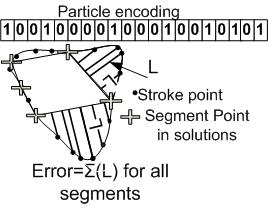
\includegraphics[scale=0.8]{images/pso1.eps}			
	\caption{AlgS1 Error}% a) Possible dominant point b) Particle encoding  
	\label{fig:DPSOERROR}
\end{figure}
 %The error is chosen to in favor of larger than the threshold is given a -ve value to lower the value of solution otherwise the system will favor the lower number of vertices'.\\ %we will want to lower the number of vertices'. \\
%if we say that s
%Alg1:sinc
%Alg2: 
\subsubsection{Hybrid Curve Algorithm \textsl{AlgS2}}
\label{sec:PolygonDivisionAlgorithm}

The second algorithm has the same problem formulation but different fitness and error functions. It was previously introduced in  \cite{CruveDivisionSwarm} where genetic programming was used as the optimizing algorithm. The particle is represented using the arrays $P_i = \left\{ {p_{ij} \left| {j = 1,2 \cdots N} \right.} \right\}$ where $p_{ij}$ is either 0 or 1. Lets denote the segments $\widehat{x_ix_j}$ as the consecutive set of points from point $x_i,x_{i+1} \cdots,x_j$. The algorithms attempts to fit each segment $\widehat{x_ix_j}$ to both line and circle. The type of the segment is determined according to the minimum error of each fit. The final error of the solutions is the summation of error of all segments.  %The goal of the algorithm is to fit the segments between the solution vertices' into straight lines or a circular arc. 
\paragraph{Fitting segments into straight line.}
\label{sec:FittingSegmentIntoStraightLine}
According to \cite{CruveDivisionSwarm} each segment $\widehat{x_ix_j}$ given a set of points $x_i,x_{i+1} \cdots,x_j$ can be fitted into the line: $y=kx+c$ where $k$ and $c$ are the slope and the intercept of the line respectively. Equation \ref{eq:Linek} and \ref{eq:LineC} 
\begin{equation}
\label{eq:Linek}
k = \frac{{N\sum\limits_{i = 1}^N {x_i y_i }  - \sum\limits_{i = 1}^N {x_i } \sum\limits_{i = 1}^N {y_i } }}{{N\sum\limits_{i = 1}^N {x_i^2 }  - \left( {\sum\limits_{i = 1}^N {x_i } } \right)^2 }}
\end{equation}
\begin{equation}
\label{eq:LineC}
c = \frac{{\sum\limits_{i = 1}^N {x_i^2 } \sum\limits_{i = 1}^N {y_i }  - \sum\limits_{i = 1}^N {x_i } \sum\limits_{i = 1}^N {x_i y_i } }}{{N\sum\limits_{i = 1}^N {x_i^2 }  - \left( {\sum\limits_{i = 1}^N {x_i } } \right)^2 }}
\end{equation}
, where $N$ is the number of points in the segment and $(x_i, y_i)$ are the coordinate of the point $i$, are used to fit the segment $\widehat{x_ix_j}$ into the straight line.
\begin{equation}
\label{eq:ds}
 d_s  = \frac{{\sum\limits_{i = 1}^N {\left| {(kx_i  + c) - y_i } \right|} }}{{N\sqrt {k^2  + 1} }}
\end{equation}
The distance ($d_s$) (Equation \ref{eq:ds}) is the average distance from segment points $(x_i, y_i)$ to the estimated line. This distance $d_s$ is used as the error of the line approximation.
\paragraph{Fitting segments into circular arc.}
\label{sec:FittingSegmentcirculararc}
Each segment is also fitted into a circular arc $(x - a)^2  + (y - b)^2  = R^2, $ where ($a,b$) are the coordinate of the center of the circle and $R$ is the radius of the circle. They is estimated using the following set of equations: 
 
\begin{equation}
a = \frac{{b_{1}a_{22} - b_{2}a_{12}}}{\Delta},
\end{equation}
\begin{equation}
	b = \frac{{b_{2}a_{11} - b_{1}a_{21}}}{\Delta},
\end{equation}
\begin{equation}
R = \sqrt {\frac{1}{N}(\sum\limits_{i = 1}^N {x_i^2 }  - 2\sum\limits_{i = 1}^N {x_i a}  + Na^2  + \sum\limits_{i = 1}^N {y_i^2  - 2} \sum\limits_{i = 1}^N {y_i b + Nb^2 } )} ,
\end{equation}

Where 
\begin{equation}
a_{11}  = 2\left[ {\left( {\sum\limits_{i = 1}^N {x_i } } \right) - N\sum\limits_{i = 1}^N {x_i^2 } } \right]
\end{equation}
\begin{equation}
a_{12}  = a_{21}  = 2\left( {\sum\limits_{i = 1}^N {x_i \sum\limits_{i = 1}^N {y_i } }  - N\sum\limits_{i = 1}^N {x_i y_i^2 } } \right),
\end{equation}
\begin{equation}
 a_{22}  = 2\left[ {\left( {\sum\limits_{i = 0}^N {y_i } } \right)^2  - N\sum\limits_{i = 0}^N {y_i^2 } } \right]
\end{equation}
\begin{equation}
b_1  = \sum\limits_{i = 0}^N {x_i^2 } \sum\limits_{i = 0}^N {x_i }  - N\sum\limits_{i = 0}^N {x_i^3 }  + \sum\limits_{i = 0}^N {x_i } \sum\limits_{i = 0}^N {y_i^2 }  - N\sum\limits_{i = 0}^N {x_i y_i^2 } , 
\end{equation}
\begin{equation}
b_2  = \sum\limits_{i = 0}^N {x_i^2 } \sum\limits_{i = 0}^N {y_i }  - N\sum\limits_{i = 0}^N {y_i^3 }  + \sum\limits_{i = 0}^N {y_i } \sum\limits_{i = 0}^N {y_i^2 }  - N\sum\limits_{i = 0}^N {x_i^2 y_i } ,
\end{equation}

\begin{equation}
\Delta  = a_{11}b_{22}-a_{12}a_{21}.
\end{equation}
 The error of the circle estimation is measured using the distance $d_c$ which is calculated using equation \ref{eq:circleE}:
 \begin{equation}
 \label{eq:circleE}
d_c  = \frac{{\sum\limits_{i = 0}^N {\left| {\sqrt {(x_i  - a)^2  + (y_i  - b)^2 }  - R} \right|} }}{N}
\end{equation}
Thus, Equation \ref{eq:circleE} $d_c$ defines the average distance $d_c$ from the segment points $x_i,y_i$ to the estimated circle ($a,b$) and $R$.

\paragraph{Determining The Segment Type.} 
\label{sec:DeterminigSegmentType}
If the average distance $d_s$ equals zero this means that the segment$\widehat{x_ix_j}$ points is exactly the straight line approximated. If the distance ($d_c$) equals zero means that the segments point lies exactly on the circular arc estimated. But the user rarely draws an exact line or circle, so the distances are used as the fitting error. The minimum distance determines the type of the current segment, in other words if ($d_s$) is smaller than ($d_c$) then the segment is labeled as a line segment otherwise it is labeled as a circular arc. 


After each segment type is determined the particle segmentation error is computed by Equation \ref{eq:errorSwarm2} 
\begin{equation}
E=\sum\nolimits_{i = 0}^M e(D_i) 
\label{eq:errorSwarm2}
\end{equation}
where $M$ is the number of segments in the solution, $D_i$ is the  approximation error of each segment as $min(d_c,d_s)$ as computed in Equation\ref{eq:circleE}  and Equation \ref{eq:ds} \cite{CruveDivisionSwarm}. The fitness is computed by the equation \ref{eq:fitnessSwarm2} 
\begin{equation}
\max fitness(P_i ) = \frac{1}{{E \times M^k }}
\label{eq:fitnessSwarm2}
\end{equation} where $E$ is the error and $M$ is number of segments and $k$ is a parameter tweaked to get minimum number of segments. $k$ is selected to be 0.5\cite{CruveDivisionSwarm}. 

\subsubsection{Solution Refine procedures} 
%\cite{PolygonApproximationPSO} used a merge and divide algorithm after each loop of the swarm system to refine the solution but we used another enhancement method.
 After each loop in the swarm algorithm, each particle loops on the set of selected dominant points to enhance the solution. Each dominant point is checked to find if it was labeled before as a possible dominant (computed as in section \ref{sec:Preprocessing}), if not the point is moved to the nearest labeled point.
   After each loop of the swarm algorithm (\textsl{AlgS1} and \textsl{AlgS2}), each particle is refined using the following procedure. For each particle $P_i$ each dominant point $P_{ij}$ is checked to find if it was labeled before as a \textit{possible dominant point} $P_{pd}$ (computed as in section \ref{sec:Preprocessing}). If it was not labeled the point $P_{ij}$ is moved to the nearest labeled point. This ensures that all of the points generated by the DPSO are possible dominant points $P_{pd}$. After that the particles are tested to make sure that the distance between every two successive dominant point is larger than the constant $min_D$. If two points are nearer than $min_D$\footnote{ 5\% of the total stroke length} then one of the points is removed. 
   
\subsection{Choosing the Best Fit}
\label{sec:bestFit}
The two PSO algorithms produce two segmentation solutions. After that the system evaluates each solution to finally select the best segmentation. This evaluation is based on the area of both the segmentation and the input stroke. The segmentation error($E_{alg}$ )represents the sum of Square Root Error of the length from the point on the stroke to the estimated curve or line. In \textsl{AlgS2}, this error is the same as the computed error in Equation \ref{eq:ErrorSwarm1} but For the second algorithm \textsl{AlgS2} it is different than the computed error in Equation \ref{eq:errorSwarm2}. The additional computation is necessary to  compare the two segmentation fairly. The system choose the minimum segmentation as the final segmentation of this stroke. 
% The segmentation which crossponds to the minimum $E_{tot}$ is the best segmentation.  
%\begin{equation}
%\label{eq:bestFit1}
%E_{area}=A_{st}-A_{sg}
% \end{equation}
% \begin{equation}
% where $A_{st}$ is the area of the input stroke, $A_{sg}$ is area of computed segmentation, $E_{alg}$ is the Segmentation Error. 
  
\section{Hybrid Segmentation Algorithm \textsl{Alg3}}
\label{sec:BenchMarckAlgorithm}

In this research, we developed another algorithm as reference to the results obtained by the DPSO algorithms. The algorithm was first implemented by  Sezgin et al. in \cite{earlyprocess}. The algorithm is divided into the following steps: 
\begin{enumerate}
	\item Compute the curvature and the speed for each point in the stroke. 
	\item   A percentage of maximum value of the speed and curvature is used as threshold.
		\item Mark the values higher than the threshold in a new arrays $L_c$ as the list of corner points generated from the curvature curve. The list $L_s$ contains the points generated from the speed curve.
	\item Compute a confidence on each list based on the type of curve. Then sort the lists $L_s$and $L_c$ by the confidence value. 
	\item Find the intersection points in both list and generate the a Sample solution $h_{curr}$. 
	\item Use $h_{curr}$ as initial solution. Loop on the following:
	
		\begin{enumerate}
			\item Generate a new solution $h_{s}$ using $h_{curr}$ and  the first point in the $L_s$ list .
			\item Generate a new solution $h_{c}$ using $h_{curr}$ and  the first point in the $L_c$ list.
			\item Test the solutions $h_{s},h_c$ to find the minimum solution.
			\item  If $h_s$ is the minimum then add the solution a list of hybrid solutions $Solutions_{set}$ and remove the first point from the list $L_s$ then set $h_s$ as $h_{curr}$. 
			\item If $h_c$ then add the solution a list of hybrid solutions $Solutions_{set}$ and remove the first point from the list $L_c$ then set $h_c$ as $h_{curr}$. 
		\end{enumerate}
		\item Choose the final solution from the list of solutions $Solutions_{set}$ as a tradeoff between  minimum error and number of corners.  
		\item Check each segment in the solution if the solution is can be estimated as a line segment if not it is fitted using a higher level Bezire curve. 
\end{enumerate}
More details about the algorithm are in \cite{earlyprocess}.


%\section{Stroke Clustring Algorithms }
%\label{sec:ClustringAlgoirthm}
%
%When the user finishes drawing a stroke the segmentation algorithm generate a list of segments that represent this stroke. The system then groups the segments generated from the segmentation algorithm. %These segments are grouped into a symbol and tested if they can be classified into one of the known symbols. If no identification is achieved the segments are added into a list of unclassified segments. When a user draws another stroke the segmented stroke is added to the list and the process is repeated until all the segments are classified to a known symbol.\\
%
%After the user draw all strokes of the symbol he has to wait 10 seconds or press finish button beside the drawing area. The set of unrecognized strokes is grouped together along with their segmentation as input to the feature extraction process. 

\section{Feature Extraction Methods}%%Feature Set
\label{sec:FeatureExtraction}

The system uses a composite set of features which include global shape properties like Rubine feature set \cite{gestureexample12},  ink density \cite{GeometryAndDomain102}, some appearance based properties like Zernike moments \cite{HeloiseBeautification}, and some stroke based structural information like number of perpendiculars lines , number of parallel lines and types of primitives in each symbol. The following list gives details on all the features used in the system.
\subsection{Structural and geometrical Features(FS1)}
Features defines the structure of the geometrical symbol.  
%\begin{description}
% \item [Structural and geometrical Features (FS1)] 
  \begin{itemize}
	 \item \emph{Segments:} Number of segments in the symbol.
	 \item \emph{Strokes:} Number of strokes or partial strokes that created the symbols.  
		\item  \emph{Primitives:} Number of primitives in the symbol. The feature helps when identifying             symbols with mixed geometric primitives like cylinders and callouts.  
		\item \emph{Curves:} Number of curves or ellipses in the symbol. 
		\item \emph{Lines:} Number of lines in the symbol. 
		\item \emph{Perpendicular} lines Number of perpendicular lines. 
		\item \emph{Parallel} lines Number of parallel lines. 
		\item \emph{Intersections} Number of intersection between lines and curves. 
		\item \emph{T intersections} Number of T intersections. 
		\item \emph{L intersections} Number of L intersections. 
		\item \emph{X intersections} Number of X intersections.
	
		%\item[No. of holes] Number of holes in the symbols. 
\end{itemize}
%\begin{description}
%	 \item[Segments] Number of segments in the symbol.
%	 \item [Strokes] Number of strokes or partial strokes that created the symbols.  
%		\item[Primitives] Number of primitives in the symbol. The feature helps when identifying             symbols with mixed geometric primitives like cylinders and callouts.  
%		\item [Curves] Number of curves or ellipses in the symbol. 
%		\item [Lines] Number of lines in the symbol. 
%		\item [Perpendicular lines] Number of perpendicular lines. 
%		\item [Parallel lines] Number of parallel lines. 
%		\item [Intersections] Number of intersection between lines and curves. 
%		\item [T intersections] Number of T intersections. 
%		\item [L intersections] Number of L intersections. 
%		\item [X intersections] Number of X intersections.
%		
%		
%		%\item[No. of holes] Number of holes in the symbols. 
%
%\end{description}
\subsection{Rubine Feature Set (FS2)} Features introduced by Rubine\cite{gestureexample12} for single stroke gestures. These features represent the global shape of the symbol drawn. To compute the features we append all segments points into single path $ink_{path}$. The features is computed on the generated path $ink_{path}$.%then compute the features based on this path.  
\begin{enumerate}
	\item Cosine of starting angle.
	\item Sine of starting angle.
	\item Length of diagonal of bounding box. It gives an idea of the size of the bounding box).
	\item Angle of diagonal. It gives an idea of the shape of the bounding box (long, tall, square).
	\item Distance from start to end.  
	\item Total stroke length
	\item Change in Rotation( Arctan ). It gives the directional angle.
	\item Absolute rotation 
	\item Rotation squared 
	\item The maximum speed reached (squared) 
	\item Total time of stroke 
\end{enumerate}
\subsection{Statistical Features (FS3)} 
\begin{enumerate}
	\item \textsl{Zernike moments:} Zernike moments of order n\footnote{ We tried different values of n. Results show the analysis of each order.} \cite{HeloiseBeautification}. 
\end{enumerate}
\subsection{Global shape properties set (FS4)}
 Features that are composites of different geometrical and statistical symbol. These features represent the global shape of the symbol drawn.

 	\begin{itemize}
\item \emph{Size Ratio} Ratio between width to height of the symbol.
	\item \emph{Ink density} Compute the density of points inside its bounding box\cite{GeometryAndDomain102}.   
 	\item \emph{Convex Hull Area} Area of convex hull with respect to area of bounding box of symbol.
	\item \emph{Convex Hull Perimeter} Perimeter of convex hull with respect to total length of symbol.
		\item \emph{Mean Centroidal radius} The Mean of the centroidal radius which is the distance from each point in the symbol to the center of gravity.
	
	\item \emph{Mean Time difference} The mean of the time difference between each two successive points in the symbol. %Different strokes are appended to construct a single path.
	%\item [Ra]
  \end{itemize}
  
 Section \ref{sec:featuresComparisions} presents a comparative result of the different feature sets from these features.

\section{Classification}%%Feature Set
\label{sec:Classification}
The system uses support vector machine (SVM) classifier with Linear kernel (Linear kernel) \cite{libsvm}. SVM is a binary classifier that maximizes the margin between the decision boundary and the support vectors. To enable SVM to learn multi classes we used one versus one strategy for combining set of binary classifier. This strategy trains $ \frac{n(n-1)}{{2}}$ binary classifier each distinguish between only two shapes. The final result is based on a number of votes each shape has from all classifiers. We used the library implementation of LibSVM \cite{libsvm} and its implementation of the one-vs-one strategy.

\subsection{Support Vector Machines}

The foundation of Support Vector Machines (SVM) were developed by Vapnik \cite{} in 1995. It is gainig increase popularity due to the high performance and efficient implementation. The goal of SVM algorithms is to generate a sperating plane between two different classes which are represented using a set of n-dimentional vectors. The generated plane is used as a good classifier to the unseen exmaples. However, there can be more than one plane that can separates the data therefore SVM attempts to find the plane that maximize the margin (distance between classifier and nearest sample) between the two classes \ref{}. To calcuate the margin, two different hyperplanes are constructed, one plane on each side of the data, these two planes are then moved to generenate the maximum margin possilbe.  


Let us consider  a two class classification task with datapoints $x_i$ where $i=1,\cdots,m$ having corresponding labels $y_i=\pm1$ where if  $y_i=1$ if $x_i$ belonged to first class and $y_i=-1$ if $x_i$ belonged to second class. Each data  point $x_i$ is represented in $N$ dimensional input or attribule space. Let the classification plane be represented as function . 
\begin{equation}
 y=f(x)=sign(\omega \cdot x - b)
\label{eq:planeEq}
\end{equation}

 The vector $\omega$ determines th orientation of a seperation plane. The scalar $b$ determines the offeset of the plane from the orgin. Lets assume that the datatpointa re linearly seperable, i.e. there are infinitely many possible seperating planes that correctly classify the training data. Figure\ref{} illustrates two different seperating planes. It is intuitively noted from the figure that the () line is more likely to generalize more data and thus introduce less classification error. This can be geometrically characterized as plane furthest from both classes.     % Which one is preferable ? Intuitively one perfers the solid pane since small perturbations of any point would not introduce misclassifications errors. Without any information, the solid plane is more likely to generalize better on future data. Geometrically we can characterize the solid plane as being furthuret from both classes. 

The SVM problem is how to construct the plane that is furthuest from both classes. One approcah is to maximize the margin between two parallel planes supporting. A plane supports a class if all points in that class are on one side of that plane. For the points with the class label $+1$ we would like there exist $\omega$ and $b$ such that $\omega \cdot x_i\> b$ or $\omega \cdot x_i -b \> 0$  depending on the class label. Let us suppose that smallest value of $\mid \omega \cdot x_i -b\mid$ iss $\kappa$, then when $ \omega \cdot x_i -b \geq \kappa$. The argument insidee the decision function is invariant under positive rescalling so we will implicity fix a scale by requiring $\omega \cdot x_i -b \geq 1 $. For the points with class label $-1$ we similary require $\omega \cdot x_i -b \leq -1 $. To find the plane furthest from both setss, we can simply maximize the distance or margin between the support planes for each class as illustrated in Figure \ref{}. The support planes are pussshed apart untill they bump inot small number of data points ( the support vecotrs ) for each class. The support vectors in Figure \ref{} are outlined in (), 


The distance or margin between these supporting planes 
\begin{equation}
 \omega \cdot x=b+1 \\
  \omega \cdot x=b-1
\end{equation}
is 
\begin{equation}
 \gamma = \frac{2}{\parallel \omega \parallel^2}
\end{equation}
Thus maximizing the margin is equivalent to minimizing $\frac{{\parallel \omega \parallel}^2}{2}$ int the following quadratic program 


\begin{equation}
 \min_{\omega,b}  \frac{{\parallel \omega \parallel}^2}{2}
\end{equation}
\begin{equation}	
\begin{array}{cc}
 s.t. \ \ \   \omega \cdot x_i \geq b+1 &    y_i \in Class 1 \\ 
 \ \ \ \ \ \   \omega \cdot x_i \leq b-1 &    y_i \in Class -1 
  \end{array} 
\end{equation}

The constrain can be simplified to $y_i(\omega \cdot x_i-b)\geq 1$. 


The margin depends on the Support vecotrs that are bumpt into the planes.  This is a primal problem Quadratic Programming (QP) problem. The concept of duality can also upsed to wields the problem to a  Largrnigian dual QP problem in Equation \ref{eq:dual}. 
% maximumm margin between parallel 
\begin{equation}
\begin{array}{c}
\min_{\alpha} \ \ \   \frac{1}{2} \sum_{i=1}^{m}{\sum_{j=1}^{m}{y_iy_j\alpha_i\alpha_jx_ix_j}} - \sum_{i=1}^{m}{\alpha_i} \\
s.t. \ \ \sum_{i=1}^{m}{y_i\alpha_i}=0   \\
  \alpha_i \geq 0  \ \ \ i=1,\cdots , m 
  \end{array} 
\label{eq:dual}
\end{equation}
Both the dual form and the primal form weilds to the same plane $\omega=\sum_{i=1}^{m}y_i\alpha_i x_i$ and threshold $b$ determined by the support vectors (for which $\alpha_i\geq 0$). 

\subsubsection{Theoretcical foundation}
From a statistical learning theory perspective these QP formulation are well founded Rougly, Statistical Learning proves that bounds on the generalization error on future points not in the training set can be obtained. Theses bounds are a function fo misclassiffied error on the training data and tersm sthat measure the complexity or capacity fo classifcation function . For linear functions, maximizing the margin of seperation as discussed abouve reduces th efunction capacilty or complexity. Thus, by explicity maximizing the margin we are minimizing bound on the generalition error and can expect better generalization with high probability. The size of the margin is not directly dependent on the dimensionaliuty of the data. Thus, we can expect good performance event for very high dimensional data (i.e, with a very large number of attribute). In a sense, problems caused by oer fitting of high - dimensional data are greatly reduced. The problem is refered to the large volume of literature in, e.g., \cite{} for more technical discussion of the taht statistical theroy. 

We can gain inishgit into thesse result susing geomertic arguments. Classification function hat have capcity to fit the training data are more likely to overfit  resulting in poor generalization.  

\subsubsection{Linearly in seperable case}
 So far we have assumed that the two datasets are linearly separable. Th this is not true, the startegy of constructing the plane that bisect the two closest points of the convex hulls will fail. As illustrated in Figure \ref{}, if the points are not linearly seperable the primal supporitng plane will fails. Since the QP task is not feasible for ethe linearly inseperable case , then we need to relax the constrains. Consider the linear inseperable problem in Figure\ref{}, Ideally we would like no points to be missclassified and no points to fall in the margin. But we must relax the constrain that insure that each point in on the approiate side of tis supporitng plane. Any point fallihng on the wrong side of tis supprting plane is considered to be an error. We want to maximize the margin and minimize the error. 
 
 This could be accomplished through minor change in the supporging plane QP problem. A nonegative slack or error variable $z_i$ is added to each constraint and then added as weighted penalty term in the objective as follows:
 \begin{equation}
 \begin{array}{c}
\min_{w,b,z}  \quad \frac{{\parallel \omega \parallel}^2}{2}+C \sum_{i=1}^{l}z_i  \\
s.t.  \quad y_i(\omega \cdot x_i -b)+z_i \geq 1  \\
    z_i \geq 0  i=1,\cdots,m
\end{array} 
\label{eq:inseperable}
\end{equation} 

Once again the primal relaxed supprting plane method is equivilent to the dual problem. The Largangian dual of the QP task is :

\begin{equation}
\begin{array}{c}
\min_{\alpha} \ \ \   \frac{1}{2} \sum_{i=1}^{m}{\sum_{j=1}^{m}{y_iy_j\alpha_i\alpha_jx_ix_j}} - \sum_{i=1}^{m}{\alpha_i} \\
s.t. \ \ \sum_{i=1}^{m}{y_i\alpha_i}=0   \\
 C \geq \alpha_i \geq 0  \ \ \ i=1,\cdots , m 
 \end{array} 
\label{eq:dual}
\end{equation}



\subsubsection {Non linear function Using Kernels}
If we consider a classification problem that cannot be seperated using a linear space (See Figure \ref{} ). A quadratic or  cubic function will work better in some casses. A classific method of converting a linear classification algoirhtm inot a nonolinear classification algoorithm is to simply add addional attribute to the data that are nonlinear functions of the original data. Existing linar classification algorithms can be then applied to the expanded dataset feature space producing non linear functions in the original input space. To construct a quadratic disceriminant in a two dimensional vector space with attributes $r$ and $s$, simply map the original two dimensional input space $\left[r,s\right]$ to the five dimensional features space $\left[r,s,rs,r^2,s^2\right]$ and construct a linear discriminiant in that space. specifically, define : $\vartheta(x):R^2  \rightarrow R^5$ then 
\begin{equation}
\begin{array}{l}
	x=[r,s] \\
	\omega \cdot x=\omega_1 r+ \omega_2 s \\
	\downarrow \\
	\vartheta(x)=\left[r,s,rs,r^2,s^2\right] \\
	
	 \omega \cdot \vartheta(x)= \omega_1 r+ \omega_2 s + \omega_3 rs+ \omega_4 r^2+\omega_5 r^2 
\end{array}
\label{eq:kernel}
\end{equation}  
The resulting classification function, 
\begin{equation}
\begin{array}{l}
f(x)=sign\left( \omega \cdot\vartheta(x)-b \right) \\
= sign\left( \omega_1 r+ \omega_2 s + \omega_3 rs+ \omega_4 r^2+\omega_5 r^2 -b \right) 
\end{array}
\label{eq:kern2}
\end{equation}  
is linear in the mapped five dimensional feature space but is quadratic in the two dimensional input space. 

For higher dimentional datasets, this nonlinear mapping method has two potential problems stemming from the fact taht dimensionality of the feature space explones exponentially. The first problem is that overfitting becomes a problem. SVM are largely immune to this porlblem since they rely on margin maximization. Provided an appropriate value of paaramter $C$ is chosen. The second concern is that it is not practical to actually compute $\vartheta(x)$. SVMs get around this issue through teh use of kernels. 

Exampine what happens when athe nonlinear mapping is introduced to equation \ref{eq:dual}. Let us define : $\vartheta(x):R^2\rightarrow R^5 \quad n^\'>> n$  we need to optimize

\begin{equation}
\begin{array}{c}
\min_{\alpha} \ \ \   \frac{1}{2} \sum_{i=1}^{m}{\sum_{j=1}^{m}{y_iy_j\alpha_i\alpha_j\vartheta(x_i)\vartheta(x_j)}} - \sum_{i=1}^{m}{\alpha_i} \\
s.t. \ \ \sum_{i=1}^{m}{y_i\alpha_i}=0   \\
 C \geq \alpha_i \geq 0  \ \ \ i=1,\cdots , m 
 \end{array} 
\label{eq:dualkernel}
\end{equation}
Notice that the mapped data only occurs as inner product in the objective. Now we apply a little mathematically rigorous magie known as hilbern schmidt kernels, first applied to SVMs in \cite{}.  By Mercer's theorem, we knoew that for ccertain mapping $\theta$ and any two points $u$ and $v$, the inner product of the the mapped points can be evalutated using the kernel function without ever explicity knowing ht emapping , e.g., $\theta(u)\theta(v)\equiv K(u,v)$. Some of the more popular known kernels are given below. New kernel are being developed to fit domian specific requriments. 

\begin{equation}
\begin{array}{cc}
\underline{\vartheta(u) & K(u,v)} \\ 
Degree d polynomial  & \left(u\cdot v +1\right)^d \\
Radial Basis Function & \exp \left( - \frac{\left\|u-v\right\|^2}{2\sigma}\right) \\
Two layer Neural Network & sigmoid \left(\eta\left(u\cdot v +1\right)+c\right) 
  \end{array} 
\label{eq:diffkernel}
\end{equation}
 
%The foundations of Support Vector Machines (SVM) have
\subsubsection{Summary of SVM}
The resulting SVM method can be summarized as follows 
\begin{enumerate}
	\item Select paramter C representign the tradeoff between minimizign the training set error and maximizing the margin. Select the kernel function and any kernel paramters. For example for the radial basis function kernel, one must select width of the gaussian $\gamma$. 
	\item Solve dual QP Equation \ref{} or an alterantive SVM formulation using an approriate quadratic programming or linear programming alogrithm. 
	\item Recover th primal threshold variable $b$ using the support vectors. 
	\item Classify new points using $f(x)=sign\left(\sum{i}y_i\alpha_i K\left(x,x_i\right)-b\right)$
\end{enumerate}

The paramters in step 1. are selected using cross valiation if sufficent data are avaliable. %However, recent model  selectin strategies can 

\subsubsection{ SVM in Machine Learning }

\subsubsection { SVM vs. Other Learning Methods}


% whate is support vector machines 
%%The classifcation problem can be restricted to consideration of the two-class problem
%without loss of generality. In this problem the goal is to separate the two classes by a
%function which is induced from available examples. The goal is to produce a classifier
%that will work well on unseen examples, i.e. it generalises well. Consider the example
%in Figure 2.1. Here there are many possible linear classifiers that can separate the data,
%but there is only one that maximises the margin (maximises the distance between it
%and the nearest data point of each class). This linear classifier is termed the optimal
%separating hyperplane. Intuitively, we would expect this boundary to generalise well as
%opposed to the other possible boundaries.
%
%Let $x_i$ , $i$ = $1.2 \dots,N$ , be the feature vectors of the training set, $X$ . These
%belong to either of two classes that are linearly spereable $\omega_1=1$ and  $\omega_2=-1$.
%The goal, is to design a hyperplane which solve the equation 
%\begin{equation}
%g(x) = \omega^{T} x + \omega g = 0
%\label{eq:svmhyper}
%\end{equation}
 % Vladimir N. Vapnik. Statistical Learning Theory. John Wiley & Sons, Inc., New
% York, NY, September 1998.
 
 %The above is a classic example of a linear classifier, i.e., a classifier that separates a set of objects into their respective groups (GREEN and RED in this case) with a line. Most classification tasks, however, are not that simple, and often more complex structures are needed in order to make an optimal separation, i.e., correctly classify new objects (test cases) on the basis of the examples that are available (train cases). This situation is depicted in the illustration below. Compared to the previous schematic, it is clear that a full separation of the GREEN and RED objects would require a curve (which is more complex than a line). Classification tasks based on drawing separating lines to distinguish between objects of different class memberships are known as hyperplane classifiers. Support Vector Machines are particularly suited to handle such tasks. 





% how decisions is made
%  how training is done 
% how testing is donel. 
% kernels 
% how multi classifier are implemented 
% how parameter for cost is measured. 
% advantages 
% disadavantages 
% importance and applications used in it. 


\section{Step by Step Example}
\label{secstepExample}
In this section a step by step example is presented to clearify the presented sytesm. Let us make an assumption that the user will draw a clock using two strokes. Figure \ref{} show the two stroke and how the user draw them. The next steps demonstrate how ouput of the system after each step 

\begin{landscape}
\begin{scriptsize}

%\begin{table}
	%\centering 

%\scalebox{0.6}{		
\begin{longtable}{|p{2cm}|p{2cm}|p{2cm}|p{2cm}|p{13cm}|}
	\caption{StepsStroke1}
	\label{tab:StepsStroke1} \\

\hline 
\multicolumn{1}{|p{2cm}|}{\textbf{Step}} & 
\multicolumn{1}{p{2cm}|}{\textbf{Discription}} &
 \multicolumn{1}{p{2cm}|}{\textbf{Inputs}} &
 \multicolumn{1}{p{2cm}|}{\textbf{Details}} &
 \multicolumn{1}{p{13cm}|}{\textbf{Output}} 
\\ \hline 
\endfirsthead

\hline
\multicolumn{3}{c}%
{{\bfseries \tablename\ \thetable{} -- continued from previous page}} \\
\multicolumn{1}{|p{2cm}|}{\textbf{Step}} & 
\multicolumn{1}{p{2cm}|}{\textbf{Discription}} &
 \multicolumn{1}{p{2cm}|}{\textbf{Inputs}} &
 \multicolumn{1}{p{2cm}|}{\textbf{Details}} &
 \multicolumn{1}{p{13cm}|}{\textbf{Output}} 
\\ \hline 
\endhead


 
%Step & Discription of Step & Input & Steps & Output \\ \hline
Stroke 1 & Extracting point and computing boundary data & -- &  see Section \ref{sec:Preprocessing} & 
\begin{scriptsize}
Stroke has 62 points = [P(198.0,153.0), P(197.0,150.0), P(197.0,145.0), P(198.0,140.0), P(203.0,125.0), P(205.0,120.0) , P(205.0,117.0), P(210.0,111.0) , P(214.0,103.0) , P(219.0,97.0), P(225.0,89.0) , P(229.0,85.0) , P(242.0,77.0) , P(247.0,73.0) , P(275.0,64.0) , P(287.0,62.0) , P(325.0,62.0) , P(333.0,63.0) , P(362.0,68.0) , P(372.0,72.0) , P(391.0,77.0) , P(406.0,83.0) , P(424.0,91.0) , P(440.0,100.0), P(474.0,133.0) , P(485.0,149.0) , P(492.0,164.0) , P(499.0,182.0) , P(501.0,191.0) , P(501.0,207.0) , P(499.0,222.0) , P(496.0,239.0) , P(471.0,292.0) , P(467.0,302.0) , P(456.0,315.0) , P(441.0,329.0) , P(427.0,339.0) , P(418.0,344.0) , P(398.0,354.0) , P(336.0,371.0) , P(283.0,376.0) , P(263.0,378.0) , P(242.0,378.0) , P(232.0,376.0) , P(213.0,373.0) , P(194.0,367.0) , P(177.0,362.0) , P(138.0,343.0) , P(129.0,336.0) , P(124.0,331.0) , P(120.0,321.0) , P(115.0,310.0) , P(113.0,297.0) , P(112.0,284.0) , P(114.0,256.0) , P(121.0,219.0) , P(128.0,202.0) , P(137.0,184.0) , P(143.0,172.0) , P(154.0,161.0) , P(172.0,146.0) , P(172.0,146.0)]

 Bonding box is  = Corner P(112.0, 62.0), w= 389.0, h=  316.0
 number of point in this stroke is   62
\end{scriptsize}
 \\ \hline
Possible Dominate point Extraction & Computing and for details see Section\ref{sec:Preprocessing} &  Stroke points  & 1. compute   the pdp  &    Number of $P_{dp}$  = 11
 Pdp = [ 2 (197.0 , 145.0 ), 4 (203.0 , 125.0 ), 3 (198.0 , 140.0 ), 22 (424.0 , 91.0 ), 19 (372.0 , 72.0 ), 26 (492.0 , 164.0 ), 28 (501.0 , 191.0 ), 9 (219.0 , 97.0 ), 31 (496.0 , 239.0 ), 0 (198.0 , 153.0 ), 41 (263.0 , 378.0 )]

\\ \hline 
Segmentation & Segmentation of Ellipse & $P_{dp}$   &  Ellipse fitting  & 
 Segmented as Ellipse with dimensions  a = 194.5 ,b = 194.5 , Center( 306.5,  220.0 )   with Error =  2.276869953758031 , Percent =0.9093857875960022
 certainty  =  0.1997008626019765 
\\ \hline
 
Stroke 2 & Extracting point and computing boundary data & -- &  see Section \ref{sec:Preprocessing} &
\begin{scriptsize}
Stroke has 205 points = [P(201.0,179.0) , P(202.0,180.0) , P(202.0,182.0) , P(202.0,185.0) , P(202.0,187.0) , P(202.0,190.0) , P(202.0,192.0) , P(202.0,196.0) , P(202.0,202.0) , P(201.0,206.0) , P(200.0,219.0) , P(198.0,231.0) , P(198.0,234.0) , P(198.0,238.0) , P(197.0,244.0) , P(197.0,248.0) , P(197.0,251.0) , P(196.0,258.0) , %P(196.0,260.0) , P(196.0,263.0) , P(195.0,265.0) , P(195.0,266.0) , P(195.0,269.0) , P(195.0,271.0) , P(195.0,273.0) , P(195.0,278.0) , P(195.0,279.0) , P(195.0,281.0) , P(195.0,282.0) , P(195.0,284.0) , P(195.0,285.0) , P(195.0,288.0) , P(195.0,290.0) , P(195.0,295.0) , P(195.0,297.0) , P(195.0,298.0) , P(196.0,298.0) , P(196.0,299.0) , P(196.0,300.0) , P(196.0,301.0) , P(197.0,301.0) , P(198.0,301.0) , P(200.0,301.0) , P(203.0,301.0) , %P(206.0,301.0) , P(208.0,301.0) , P(213.0,301.0) , P(217.0,302.0) , P(219.0,302.0) , P(223.0,303.0) , P(234.0,304.0) , P(237.0,304.0) , P(240.0,306.0) , P(246.0,306.0) , P(247.0,307.0) , P(248.0,307.0) , P(249.0,307.0) , P(250.0,307.0) , P(250.0,306.0) , P(250.0,305.0) , P(250.0,304.0) , P(250.0,302.0) , P(251.0,299.0) , P(251.0,296.0) , P(251.0,294.0) , P(251.0,289.0) , P(252.0,285.0) , P(253.0,279.0) , P(253.0,274.0) , P(253.0,271.0) , P(253.0,264.0) , P(253.0,257.0) , P(254.0,252.0) , P(254.0,241.0) , P(254.0,237.0) , P(255.0,232.0) , P(255.0,229.0) , P(255.0,225.0) , P(256.0,212.0) , P(256.0,209.0) , P(256.0,206.0) , P(257.0,205.0) , P(257.0,200.0) , P(257.0,197.0) , P(258.0,195.0) , P(258.0,194.0) , P(258.0,189.0) , P(258.0,187.0) , P(258.0,186.0) , P(259.0,184.0) , P(259.0,181.0) , P(259.0,179.0) , P(259.0,178.0) , P(260.0,176.0) , P(260.0,174.0) , P(260.0,173.0) , P(260.0,172.0) , P(260.0,171.0) , P(260.0,169.0) , P(260.0,168.0) , P(260.0,167.0) , P(261.0,166.0) , P(261.0,165.0) , P(261.0,164.0) , P(261.0,162.0) , P(262.0,162.0) , P(263.0,162.0) , P(264.0,162.0) , P(268.0,162.0) , P(275.0,162.0) , P(279.0,162.0) , P(289.0,162.0) , P(291.0,162.0) , P(301.0,163.0) , P(305.0,164.0) , P(312.0,164.0) , P(315.0,165.0) , P(318.0,165.0) , P(319.0,165.0) , P(319.0,166.0) , P(320.0,168.0) , P(320.0,171.0) , P(320.0,173.0) , P(320.0,176.0) , P(321.0,182.0) , P(321.0,191.0) , P(322.0,198.0) , P(322.0,211.0) , P(323.0,226.0) , P(324.0,229.0) , P(324.0,238.0) , P(324.0,263.0) , P(325.0,272.0) , P(325.0,281.0) , P(325.0,288.0) , P(325.0,291.0) , P(325.0,297.0) , P(325.0,299.0) , P(325.0,301.0) , P(325.0,305.0) , P(324.0,306.0) , P(324.0,307.0) , P(323.0,308.0) , P(324.0,307.0) , P(325.0,307.0) , P(328.0,306.0) , P(332.0,306.0) , P(339.0,306.0) , P(347.0,305.0) , P(354.0,304.0) , P(365.0,304.0) , P(376.0,304.0) , P(379.0,304.0) , P(385.0,304.0) , P(391.0,304.0) , P(392.0,304.0) , P(393.0,304.0) , P(393.0,302.0) , P(393.0,301.0) , P(394.0,297.0) , P(394.0,290.0) , P(393.0,284.0) , P(393.0,274.0) , P(392.0,258.0) , P(391.0,245.0) , P(391.0,233.0) , P(389.0,213.0) , P(388.0,198.0) , P(388.0,189.0) , P(388.0,184.0) , P(388.0,178.0) , P(388.0,177.0) , P(388.0,176.0) , P(388.0,174.0)
.................................................................................................................. .................................................................................  , P(388.0,173.0) , P(388.0,171.0) , P(388.0,170.0) , P(388.0,168.0) , P(388.0,167.0) , P(388.0,166.0) , P(388.0,165.0) , P(389.0,165.0) , P(390.0,165.0) , P(395.0,165.0) , P(401.0,165.0) , P(406.0,165.0) , P(418.0,166.0) , P(424.0,167.0) , P(426.0,167.0) , P(429.0,167.0) , P(430.0,167.0) , P(431.0,167.0) , P(432.0,167.0) , P(433.0,169.0) , P(434.0,170.0) , P(434.0,174.0) , P(436.0,185.0) , P(440.0,200.0) , P(442.0,220.0) , P(442.0,224.0) , P(446.0,267.0) , P(447.0,279.0) , P(448.0,286.0) , P(448.0,287.0) , P(448.0,287.0)]

 Bonding box is  = Corner P(195.0, 162.0), w= 253.0, h=  146.0
 \end{scriptsize}
  \\ \hline
  & Possible Dominate point Extraction for details see Section\ref{sec:Preprocessing} &  Stroke points  & 1. compute the $P_{pd}$  & \begin{scriptsize}   Number of $P_{pd}$  =  36

 Pdp = [ 25 (195.0 , 278.0 ), 30 (195.0 , 285.0 ), 33 (195.0 , 295.0 ), 27 (195.0 , 281.0 ), 34 (195.0 , 297.0 ), 46 (213.0 , 301.0 ), 47 (217.0 , 302.0 ), 50 (234.0 , 304.0 ), 28 (195.0 , 282.0 ), 94 (260.0 , 174.0 ), 93 (260.0 , 176.0 ), 95 (260.0 , 173.0 ), 98 (260.0 , 169.0 ), 48 (219.0 , 302.0 ), 99 (260.0 , 168.0 ), 109 (275.0 , 162.0 ), 113 (301.0 , 163.0 ), 94 (260.0 , 174.0 ), 132 (325.0 , 272.0 ), 136 (325.0 , 297.0 ), 112 (291.0 , 162.0 ), 137 (325.0 , 299.0 ), 110 (279.0 , 162.0 ), 144 (325.0 , 307.0 ), 147 (339.0 , 306.0 ), 150 (365.0 , 304.0 ), 132 (325.0 , 272.0 ), 168 (388.0 , 189.0 ), 171 (388.0 , 177.0 ), 174 (388.0 , 173.0 ), 146 (332.0 , 306.0 ), 175 (388.0 , 171.0 ), 183 (395.0 , 165.0 ), 186 (418.0 , 166.0 ), 169 (388.0 , 184.0 ), 191 (431.0 , 167.0 ) ] 

  \end{scriptsize}
    \\ \hline
 \\ \hline 
Segmentation & Segmentation of Ellipse & $P_{dp}$   &  Ellipse fitting  & 
  The Ellipse is   a = 125.5 ,b = 125.5 , Center( 320.5,  235.0 )   with Error =  7.074966523515405 , Percent =1.1481777694994926 certainty  =  0.08114368920921669  
 \\ \hline
 Segmentation & PSO Segmentation ALgS1 & $P_{dp}$  & ALgS1 &   Particles =  [  1 0 1 0 0 1 1 1 1 1 1 0 0 0 1 0 0 0 1 ] 
 The particle  Particles =  [  1 0 0 0 0 0 0 0 0 0 0 0 0 0 0 0 0 0 0 0 0 0 0 0 0 0 0 1 0 0 0 0 0 0 0 0 0 0 0 0 0 0 0 0 0 0 0 0 0 0 1 0 0 0 0 0 0 0 0 0 0 0 0 0 0 0 0 0 0 0 0 0 0 0 0 0 0 0 0 0 0 0 0 0 0 0 0 0 0 0 0 0 0 0 1 0 0 0 0 0 0 0 0 0 0 0 0 0 0 0 0 0 0 0 0 0 0 0 0 0 0 0 0 0 0 0 0 0 0 0 0 0 1 0 0 0 0 0 0 0 0 0 0 0 0 0 0 0 0 0 1 0 0 0 0 0 0 0 0 0 0 0 0 0 0 0 0 0 1 0 0 0 0 0 0 0 0 0 0 0 0 0 0 0 0 0 0 0 0 0 0 1 0 0 0 0 0 0 1 0 0 0 0 1 0 ] 
 
 First Polygonization PSO = [[[  S0 Line[P(201.0,179.0) to P(195.0,281.0)]  ,      S1 Line[P(195.0,281.0) to P(234.0,304.0)]  ,      S2 Line[P(234.0,304.0) to P(260.0,174.0)]  ,      S3 Line[P(260.0,174.0) to P(325.0,272.0)]  ,      S4 Line[P(325.0,272.0) to P(365.0,304.0)]  ,      S5 Line[P(365.0,304.0) to P(388.0,189.0)]  ,      S6 Line[P(388.0,189.0) to P(431.0,167.0)]  ,      S7 Line[P(431.0,167.0) to P(442.0,220.0)]  ]]]  
 \\ \hline 
 
 
 
		\end{longtable}
%}

%\end{table}

\end{scriptsize}

\end{landscape}

%\begin{enumerate}
%\begin{itemize}
	
	
%	\item Processing for the first Stroke 1.  
	
%	\item Possible Dominiate Point Extraction
%	\item Segmentation 
%	   Computing 
%	\begin{enumerate}
%	\item Ellipse detection  
%	      Calcualting estimated ellipse with radius = $\frac{w}{2}$  and center as same as the bounding box of stroke.  
%	      The ouput of the system $$
% \end{enumerate}
%	
%	
%\end{enumerate}
%  
%
%\end{itemize}